\documentclass{article}
\usepackage[utf8]{inputenc}
\usepackage{amsmath}
\usepackage{listings}
\usepackage[norsk]{babel}
\usepackage{graphicx}
\usepackage{float}
\usepackage{listings}
\usepackage{xcolor}

% Define colors
\definecolor{mygreen}{rgb}{0,0.6,0}
\definecolor{mygray}{rgb}{0.5,0.5,0.5}
\definecolor{mymauve}{rgb}{0.58,0,0.82}

% Define the R language style
\lstdefinestyle{Rstyle}{
  language=R,
  basicstyle=\ttfamily,
  keywordstyle=\color{blue},
  commentstyle=\color{mygreen},
  numberstyle=\tiny\color{mygray},
  stringstyle=\color{mymauve},
  breaklines=true,
  showstringspaces=false,
  numbers=left,
  frame=single,
}

\title{Oblig 1b: Analyse av Terningdropp}
\author{Gormery Kombo}
\date{\today}

\begin{document}

\maketitle

\section{Introduksjon}
I denne rapporten analyserer jeg data samlet fra et eksperiment hvor en terning ble droppet fra ulike høyder. Jeg undersøker sammenhengen mellom høyden terningen ble sluppet fra (Dropp) og lengden den rullet (Lengde) etter å ha truffet bakken. Analysen inkluderer regresjonsanalyse og residualanalyse for å forstå forholdet mellom disse variablene.

\section{Oppgave 2}
\subsection{2a: Datainnsamling og Analyse}
Dataene som ble samlet inn er tilgjengelige i filen \texttt{terningDropp.csv}. Dataene ble analysert ved hjelp av R for å utføre statistiske beregninger og visuelle representasjoner.

\subsection{2b: Regresjonsanalyse for de Første 5 Målingene}
Først ble det utført en regresjonsanalyse på de første fem målingene for å estimere sammenhengen mellom 'Dropp' og 'Lengde'. Resultatene gir oss en innsikt i hvordan lengden varierer med høyden i de første forsøkene.

\begin{lstlisting}[style=Rstyle]
lm_first5 <- lm(Lengde ~ Dropp, data=df[1:5, ])
summary(lm_first5)
\end{lstlisting}
\textbf{Manuell beregning av regresjonslinjen:} 
bruker følgende formel for manuell beregning:

\begin{align*}
\beta &= \frac{n\sum(xy) - \sum x \sum y}{n\sum(x^2) - (\sum x)^2} \\
\alpha &= \bar{y} - \beta\bar{x}
\end{align*}

Beregner summene:
\begin{align*}
\sum x &= 188 \\
\sum y &= 326 \\
\sum xy &= 13500 \\
\sum x^2 &= 7674
\end{align*}

Deretter beregner vi \( \beta \) og \( \alpha \):
\begin{align*}
\beta &= \frac{5 \times 13500 - 188 \times 326}{5 \times 7674 - 188^2} \\
\alpha &= \frac{326}{5} - \beta \times \frac{188}{5}
\end{align*}

\textbf{Sammenligning:} 
Sammenlign de manuelt beregnede verdiene av \( \alpha \) og \( \beta \) med de fra R-utdataen for å sikre nøyaktighet.
R-koden gir oss \( \beta = 2.0529 \) og \( \alpha = -11.9881 \).

og manuelt beregnet gir oss: \( \beta = 2.0529 \) og \( \alpha = -11.9881 \).
\begin{figure}[H]
    \centering
    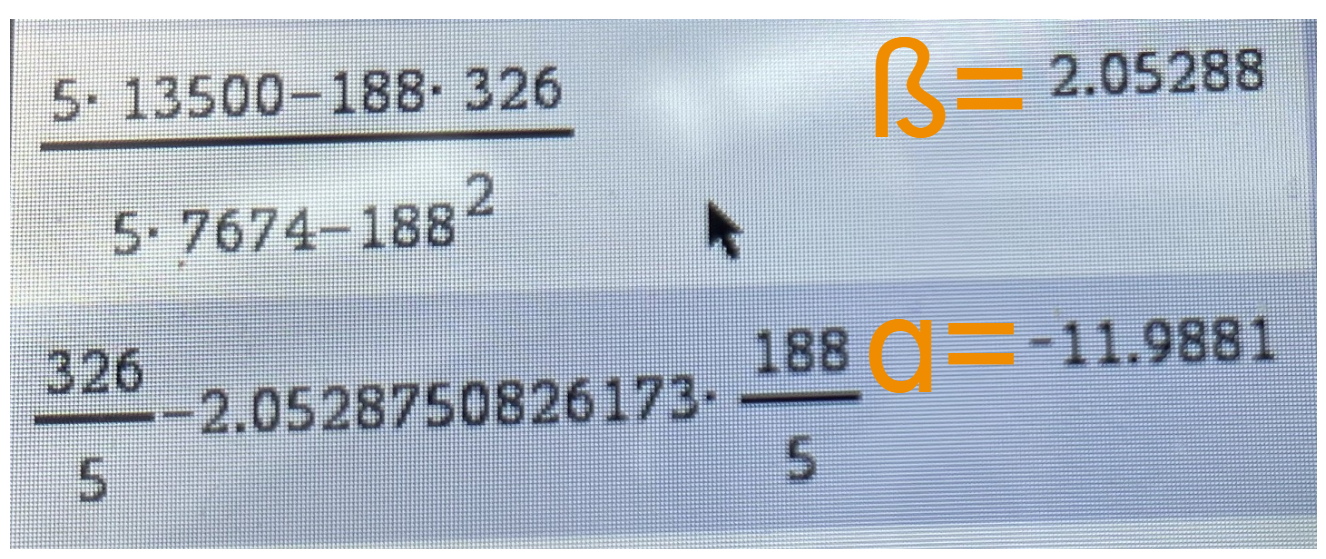
\includegraphics[width=0.8\textwidth]{manual_calculation_regresion.png}
    \caption{manuaelt beregning på kalulatoren (2b)}
\end{figure}

\subsection{2c: Regresjonsanalyse for Hele Datasettet}
Deretter ble en lignende regresjonsanalyse utført på hele datasettet for å se om det samme mønsteret holder for en større mengde data.

\begin{lstlisting}[style=Rstyle]
    lm_full <- lm(Lengde ~ Dropp, data=df)
    \end{lstlisting}

\subsection{2d: Spreddiagram av Data}
Følgende spreiddiagram viser alle datapunktene (Dropp mot Lengde) fra eksperimentet. Dette gir oss en visuell representasjon av datadistribusjonen.

\begin{figure}[H]
    \centering
    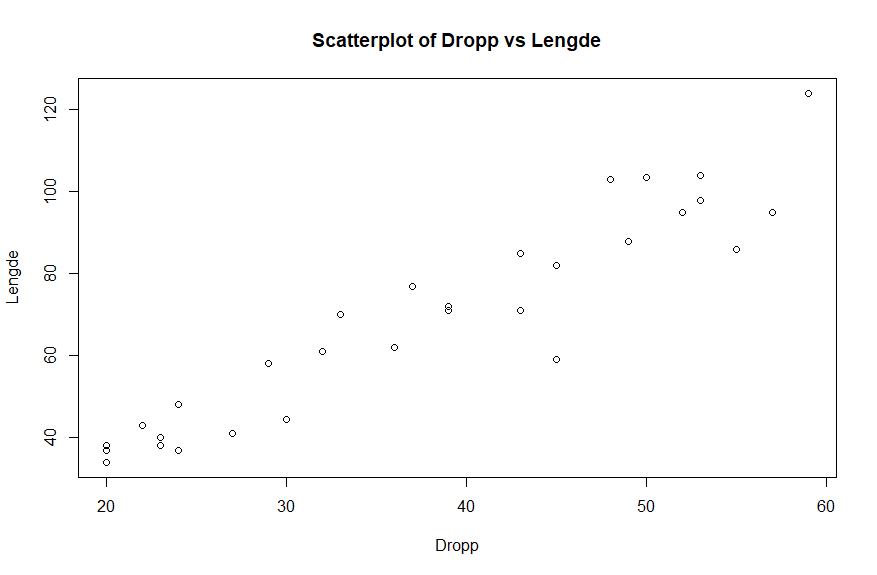
\includegraphics[width=0.8\textwidth]{Rplot03.png}
    \caption{Spreddiagram av Dropp mot Lengde (2d)}
\end{figure}

\subsection{2e: Spreddiagram med Regresjonslinje}
Dette spreiddiagrammet inkluderer regresjonslinjen som viser den estimerte lineære sammenhengen mellom 'Dropp' og 'Lengde' for hele datasettet.

\begin{figure}[H]
    \centering
    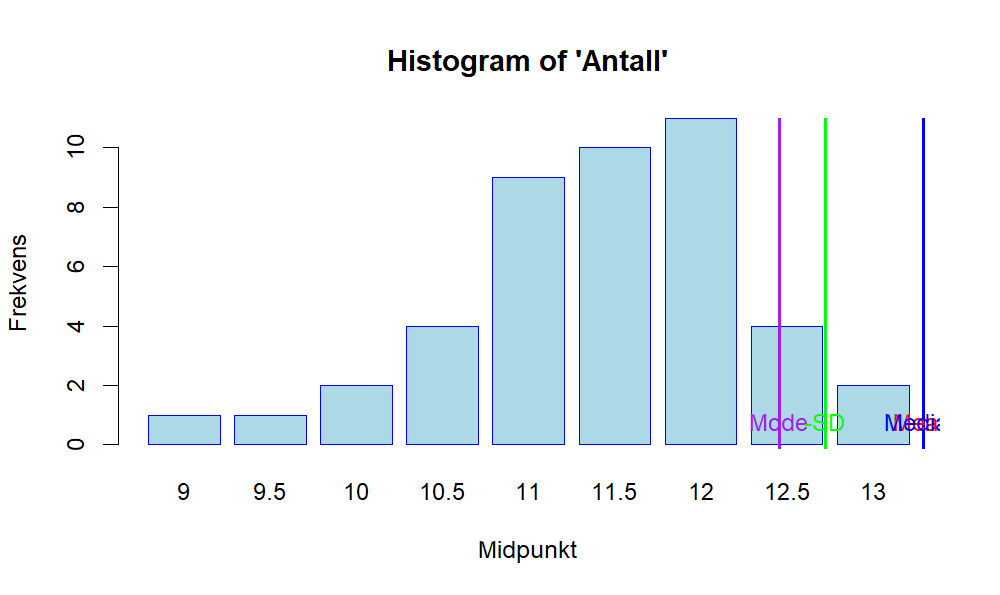
\includegraphics[width=0.8\textwidth]{Rplot02.png}
    \caption{Spreddiagram med regresjonslinje (2e)}
\end{figure}
\subsection{2g: Sum av Kvadrerte Residualer (SSe)}
Summen av de kvadrerte residualene (SSe) gir oss en kvantitativ måling av hvor godt regresjonsmodellen passer dataene. Lavere verdier indikerer en bedre passform.

\begin{lstlisting}[style=Rstyle]
ssr_first5 <- sum(residuals(lm_first5)^2)
ssr_full <- sum(residuals(lm_full)^2)
\end{lstlisting}

\subsection{2g: Sum av Kvadrerte Residualer (SSe)}
\begin{lstlisting}[style=Rstyle]
ssr_first5 <- sum(residuals(lm_first5)^2)
ssr_full <- sum(residuals(lm_full)^2)
\end{lstlisting}

\textbf{SSR (2g):} SSR gir en kvantitativ måling av hvor godt regresjonsmodellen passer dataene. Lavere verdier indikerer en bedre passform.

\textbf{Beregning:}
\[ \text{SSR for de første 5 målingene: } \sum_{i=1}^{5} (y_i - \hat{y}_i)^2 = 748.808 \]

\[ \text{SSR for hele datasettet: } \sum_{i=1}^{n} (y_i - \hat{y}_i)^2 = 2114.794 \]

Her representerer \(y_i\) de faktiske observasjonene, \(\hat{y}_i\) er de estimerte verdiene fra regresjonsmodellen, og \(n\) er antall observasjoner.

\subsection{2h: Standardfeil (se)}
Standardfeilen (SE) gir oss en idé om usikkerheten i estimatet av regresjonskoeffisientene. Den hjelper oss å forstå hvor nøyaktig vår lineære modell estimerer den avhengige variabelen.

\begin{lstlisting}[style=Rstyle]
se_first5 <- sqrt(ssr_first5 / lm_first5$df.residual)
se_full <- sqrt(ssr_full / lm_full$df.residual)
\end{lstlisting}

\textbf{Standardfeil (2h):} SE gir en indikasjon på nøyaktigheten i estimatene av regresjonskoeffisientene.

\textbf{Beregning:}
\[ \text{SE for de første 5 målingene: } SE = \sqrt{\frac{\text{SSR}}{df}} = \sqrt{\frac{748.808}{\text{df.residual\_first5}}} = 15.79882 \]

\[ \text{SE for hele datasettet: } SE = \sqrt{\frac{\text{SSR}}{df}} = \sqrt{\frac{2114.794}{\text{df.residual\_full}}} = 8.690704 \]

Her representerer \(\text{df.residual\_first5}\) og \(\text{df.residual\_full}\) frihetsgradene for residualene for henholdsvis de første 5 målingene og hele datasettet.

\subsection{2i: Lagring av Arbeid (for meg selv)}
Jeg Lagret det utførte arbeidet som en r prosject på github: \\ 
\texttt{https://github.com/valiantlynx/statistics-course/tree/main/statistikk-oblig-1b}

\end{document}
